Based on Geddes et al.'s \citeyearpar{Geddes.2014}
`Autocratic regimes' data Frantz and Kendall-Taylor
analyze 154 dictatorships over the period from 1981 to 2004.
The authors follow the example of \citet{Vreeland.2008} and
run ordered logistic regressions 
(c.f. \cite{Fox.2008,Fox.2011}) to account for the ordinal 
nature of their dependent variables. Consequently, the
research design probes the effect of co-optation on either 
type of political repression based on pooled time-series 
cross-section data. Furthermore, as institutional changes 
might take time to impact government policies, Frantz and 
Kendall-Taylor use contemporaneous levels of 
co-optation ($t_0$) to predict future levels of political 
repression ($t+1$ to $t+5$). All models include a lagged 
dependent variable ($t_0$) to account for serial 
autocorrelation and standard errors are clustered at 
the country level to counteract heteroscedasticity 
\citep{Beck.1995}. Finally, Frantz and Kendall-Taylor used
multiple imputation to avoid inefficiency and biased 
estimates or inferences 
\citep{King.2001b,Honaker.2010,Honaker.2011}. This section
introduces the three key variables involved, Appendix A 
provides summary information on all variables.

Information on political repression is drawn from two 
different sources. Empowerment rights restrictions are 
measured using Freedom House's civil liberties scale. It 
captures the extent to which citizens enjoy the ``freedoms 
of expression and belief, associational and organizational 
rights, rule of law, and personal autonomy from the state'' 
\citep{FreedomHouse.2010}. In contrast to alternative 
measurements, Frantz and Kendall-Taylor argue, the Freedom 
House data is not endogenous to the existence of political 
parties and legislatures, i.e. co-optation. The scale runs 
from $1$ to $7$, and higher values denote more restrictions 
on empowerment rights. Physical integrity violations are 
measured using the physical integrity index from the CIRI 
human rights dataset which provides ``standards-based 
measures of government human rights practices'' 
\citep[402]{Cingranelli.2010b}. It assesses the extent of 
torture, political imprisonment, extra-judicial killings, 
and disappearances on a scale from $0$ to $8$ whereby higher
values denote more government respect for the sanctity of 
person. Frantz and Kendall-Taylor recode the index such that
higher values denote more political repression.

\begin{figure}[!htb]
\centering
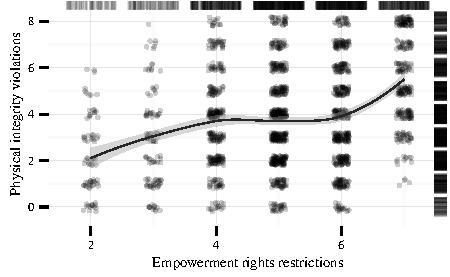
\includegraphics[width=\linewidth]{./sections/02data/scatterRepression.pdf}
\caption{Political repression in authoritarian 
regimes between 1981 and 2004. Rug plots and LOESS smoother 
with .95 per cent confidence envelope added.}
\label{fig:scatterRepression}
\end{figure}

The typology of political repression draws out meaningful
differences between authoritarian regimes. This can be seen 
from Figure \ref{fig:scatterRepression} which explores 
their relationship in the unimputed sample. The full range 
of physical integrity violations is observed, but 
empowerment rights restrictions do not take their lowest 
possible value $1$. Hence, all authoritarian regimes 
restrict civil and political liberties, but they do not 
always disrespect the sanctity of the individual. Moreover, 
Pearson's $r$ between both repression types is only  
$0.31$, and the LOESS smoother indicates that this already 
weak relationship disappears in certain regions of the data.
More precisely, the smoother stays flat across the most 
densely populated interval of empowerment rights 
restrictions ($4$ to $6$) and no inferences whatsoever may 
be drawn from changes in one type of political repression on 
the other. Consequently, although authoritarian regimes
use both types of political repression there is empirical 
reason to believe that they differ to ``the extent to
which they rely on one type more than the other'' 
\citep[336]{Frantz.2014}.

\begin{wrapfigure}{r}{0.48\textwidth}
\centering
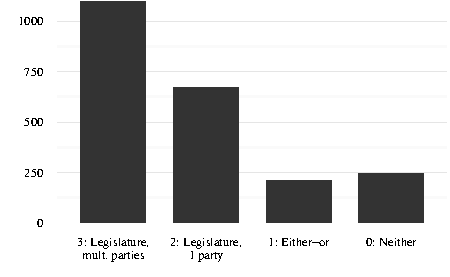
\includegraphics[width=\linewidth]{./sections/02data/barCooptation.pdf}
\caption{Co-optation, 1981-2004}
\label{fig:barCooptation}
\end{wrapfigure}
Frantz and Kendall-Taylor assume that co-optation tips the 
scales of political repression. They measure this key 
explanatory variable by the existence of political parties 
and legislatures. Information on either institution is drawn 
from the `Democracy \& Dictatorship' data 
\citep{Cheibub.2010} that map their de facto existence. 
Frantz and Kendall-Taylor create an index that takes the 
value of 3 if there is a multi-party legislature, 
2 if there is a single-party legislature, 1 if there is no 
legislature but at least one political party or, 
equivalently, if there is a non-partisan legislature, and 0 
if neither exists. The authors presume that their index 
behaves linearly, and they justify their coding scheme with 
an interest in the ``interactive effect'' of legislatures 
and political parties \citep[338]{Frantz.2014}. Figure 
\ref{fig:barCooptation} explores the empirical picture in 
the unimputed data. The majority of $2,221$ country-year 
observations falls into the highest category. Accordingly, 
more than half of all authoritarian regimes in the data 
sponsor multi-party legislatures. Single-party regimes come 
in second, and only a minority of observations ranks lower 
than $2$ on the index. In sum, the crucial empirical 
distinction is whether authoritarian regimes co-opt via 
single party or multiple parties.